\chapter{Background\label{cha:background}}

The 2010 Formula SAE vehicle is essentially made up of five functional systems, namely the \emph{engine}, \emph{transmission}, \emph{braking}, \emph{telemetry}, and \emph{driver interface} systems. The background of these systems is discussed further in this chapter, to provide the reader with the knowledge required to follow the reasoning for our design. The specific vehicle components that interface with the four electronic modules and the electro-pneumatic system are annotated in Fig. \ref{fig:background_overview_topdown}. 

\vspace{1em}
\begin{figure}[H]
\centering
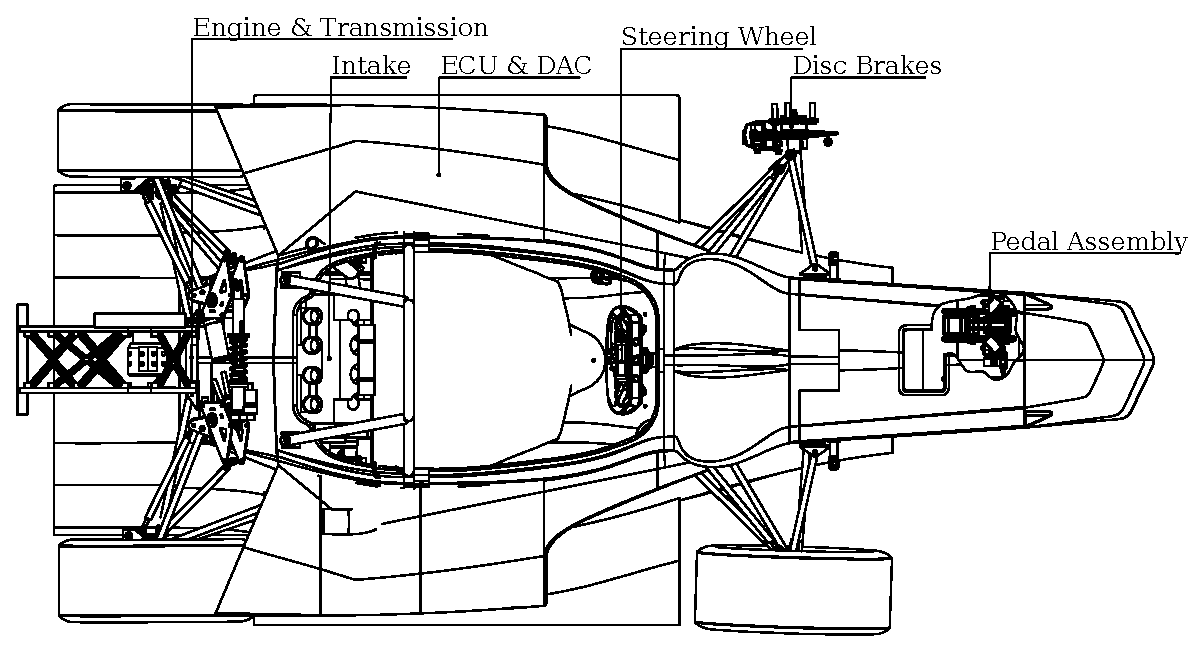
\includegraphics[width=6in,keepaspectratio]{background/figures/background_diagram.eps}
\caption{Top-down view of the 2010 Formula SAE vehicle.}
\label{fig:background_overview_topdown}
\end{figure}

\section{Engine}

\subsection{Overview}

brief {}``what is engine'', honda cbr, etc.

maximise power output (performance application)

torque power curve, etc.

\subsection{ECU}

A specialized third-party component called the \emph{Engine Control Unit} (ECU) controls the fuel injector and spark coil systems that in turn control the combustion cycle of the engine. The particular model of ECU used by the Formula SAE car is the S80Pro from DTAFast \cite{s80pro}. The ECU uses the O$_{2}$, MAP, cam position, and crank position sensors to adjust the fuel injector and spark coil timings. This keeps the engine running smoothly. The ECU features a traction control system that monitors wheel slip and cuts spark and fuel to provide traction when one of the wheels is slipping. The ECU also collects the various sensor readings and makes them available to other electronic devices at a fixed frequency through a shared data bus. 

\begin{figure}[H]
\centering
%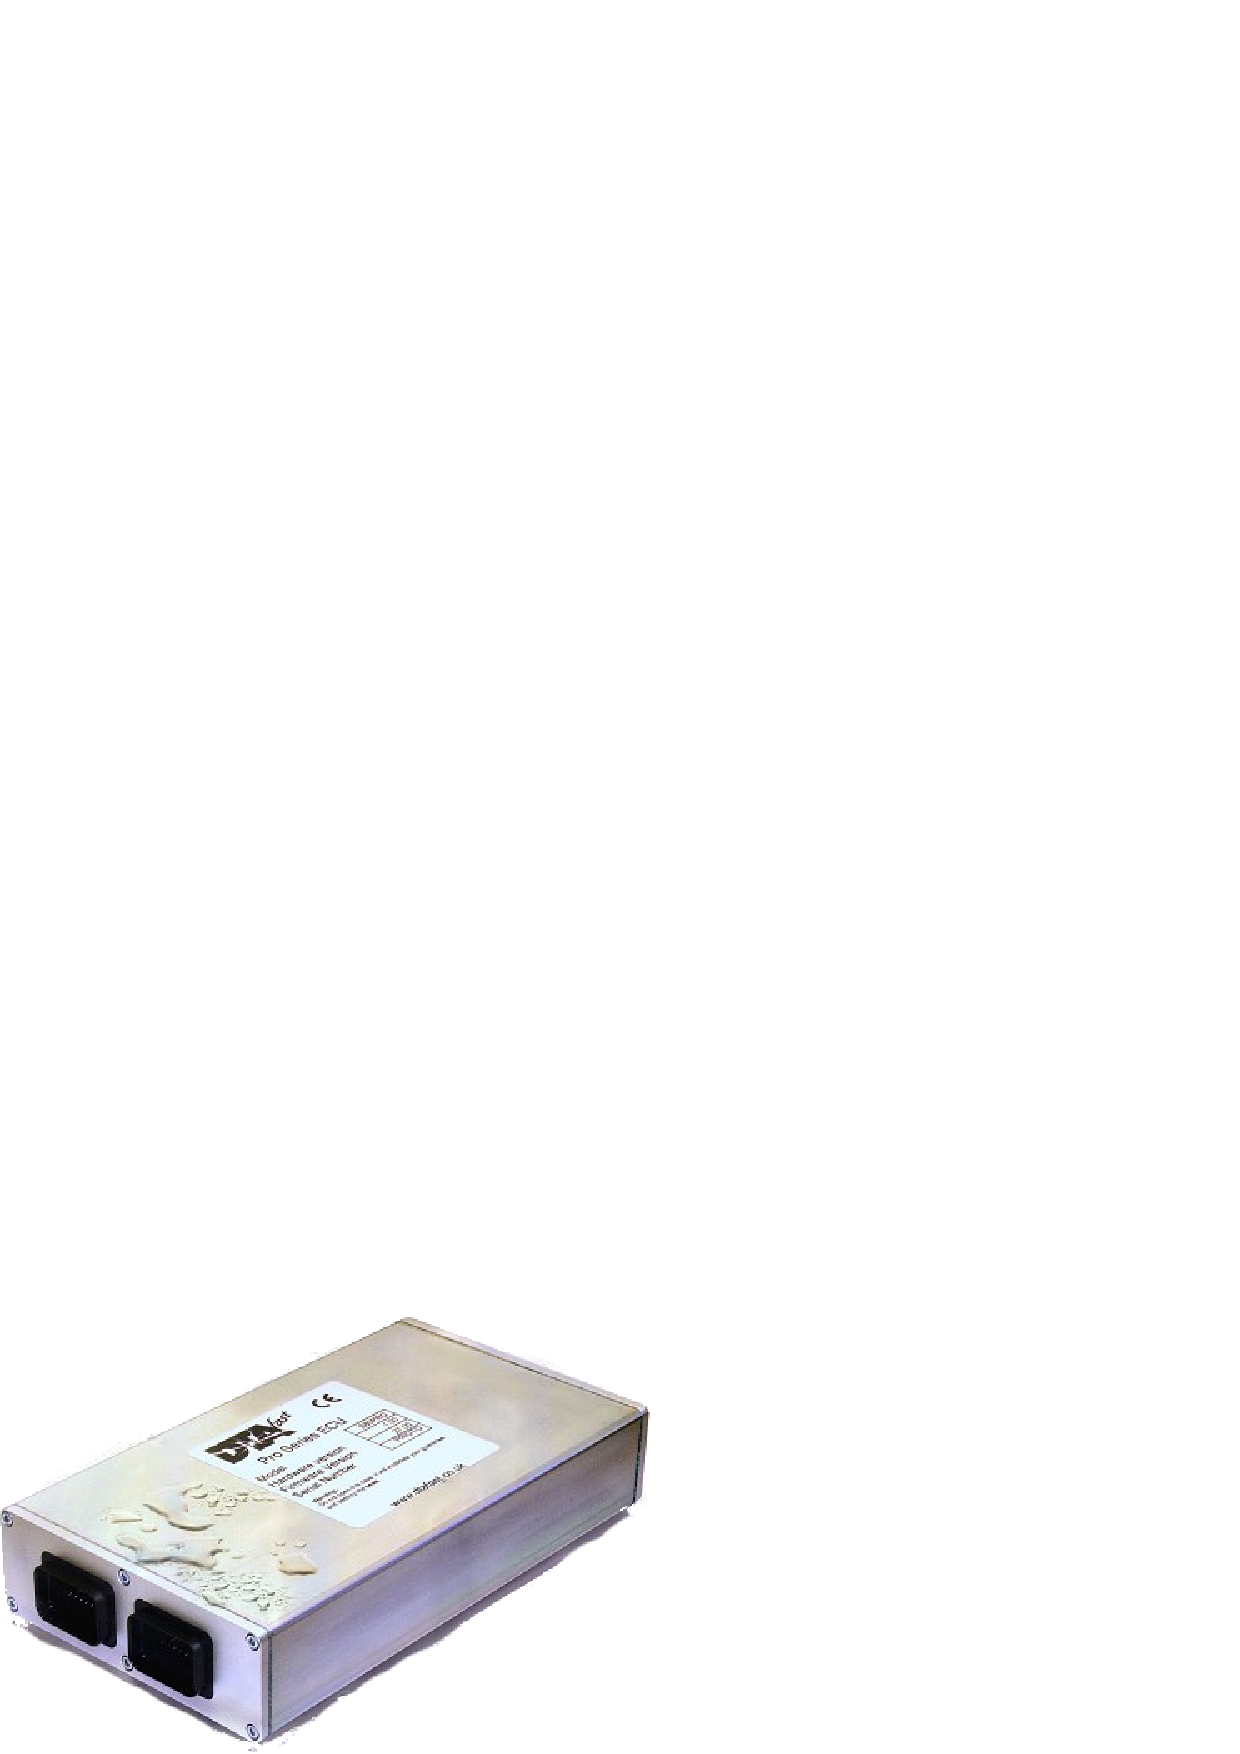
\includegraphics[scale=0.5]{Figures/s80.png}
\caption{The DTAFast S80Pro engine control unit.}
\label{fig:s80pro_product}
\end{figure}

\subsubsection{ECU Data interfaces\label{sec:background_ecu_data_interfaces}}

The ECU provides 3 digital communication methods:
\begin{itemize}
  \item An RS-232 link is used by the software that DTA provides for tuning and controlling the ECU. The serial protocol that the software uses is proprietary and undocumented.
  \item A read-only CAN bus interface that emits ECU data at a fixed frequency. The message format for the CAN data is documented in Appendix \ref{cha:ecu_can_spec}.
  \item Several CMOS-level discrete inputs:
  \begin{itemize}
    \item Launch Control toggle, which toggles the launch control feature in the ECU,
    \item Shift cut, which signals the ECU to reduce engine power before a downshift
    \item Traction control toggle, which toggles the traction control feature in the ECU,
    \item Traction control wet/dry, which switches between two different sets of traction control parameters in the ECU.
  \end{itemize}
\end{itemize}

Detailed descriptions of the ECU's launch control, shift cut, and traction control features can be found in the manual \cite{s80pro}.
 
\nomenclature{RS-232}{Recommended Standard 232, a byte-oriented serial communications protocol, typically asynchronous.}

\subsection{Intake and Exhaust}

Intake background, pressure waves, etc. Torque curve depends on length, 

\subsection{Research and Modelling of Variable Length Intake}

present research done by others on team, quantified runner length
dependence

intake length changes power

quantified length versus power on actual vehicle

chose optimal intake length

proposed variable length intake system for future work

\subsection{Starting System}

current requirements, starter motor, etc.


\section{Transmission}
\label{sec:background_transmission}

\subsection{Overview}

The Formula SAE 2010 vehicle uses a 6-speed manual sequential transmission to transmit power from the engine to the drive train. As in other types of manual transmissions, the sequential transmission works by engaging and disengaging several sets of gears with shift forks to obtain different gear ratios. A cast steel drum inside the transmission, called the \emph{shift drum}, has a series of complex grooves machined into it, in which the shift forks ride. Rotating the drum causes the forks to engage one gear and disengage the other. A ratcheting mechanism allows a single external lever, called the \emph{shift lever}, to rotate the drum forward and back by a discrete amount. Each full movement of the lever forwards or backwards causes a gear change up or down, respectively \cite{HowtoManualTransmission, cbr600}.

\subsection{Neutral Sensing}

The stock CBR600f4i engine is fitted with a simple 1-wire sensor which is connected to ground when the transmission is in neutral. The wire is left floating when the vehicle is in gear.

\subsection{Gear Position Sensing}

The stock transmission has no means of determining what gear the transmission is in; it can only determine when the transmission is in neutral using the aforementioned neutral sense wire. The ECU has provisions for reading a gear position potentiometer that can be attached to the shift drum, however this requires mechanical modification of the shift drum itself.

\subsection{Clutch}

The CBR600f4i is equipped with a multi-plate clutch which serves to transmit torque from the engine to the drivetrain. Layers of friction plates in the clutch are forced to rotate together when the clutch is engaged by a series of pre-tensioned springs. When the clutch is disengaged externally via the \emph{clutch lever}, the plates are separated and the drivetrain is allowed to spin freely from the engine. The clutch lever is actuated on the stock motorcycle with a hand lever via cable.

\subsubsection{Equations of Motion}

Equations of motion governing the clutch dynamics are:

\begin{equation}\label{eq:clutch_dynamics_a}
  J_c\dot{\omega}_c=T_c-T_d-b_c\cdot\left(\omega_c-\omega_t\right)
\end{equation}

\begin{equation}\label{eq:clutch_dynamics_b}
  \dot{T}_d=k\left(\phi_d\right)\cdot\left(\omega_c-\omega_t\right),
\end{equation}

where $J_c$ is the inertia of the clutch plates, $T_c$ the torque transmitted through the clutch, $b_c$ the clutch damping rate, and $\omega_c$ and $\omega_t$ are speeds of the clutch plates and transmission respectively \cite{clutch_control}.

A major point of interest in the operation of the clutch is the transition from fully disengaged to fully engaged, and vice-versa. In this state the clutch plates slip against each other as one rotates faster. \Citet{clutch_control} describe the torque transmitted through the clutch in slipping, $T_c{slip}$, as

\begin{equation}\label{eq:clutch_slip}
  T_c{slip}=F_n\mu R_a \cdot sgn\left(\omega_e-\omega_c\right),
\end{equation}

where $F_n$ is the normal force on the clutch plates, $\mu$ the coefficient of friction on the plate surfaces, and $R_a$ the radius of the plates, and $\omega_e$ and $\omega_c$ are the rotational velocities of the engine, and clutch discs, respectively. This shows that the amount of torque transmitted depends dynamically on the normal force $F_n$, which is proportional to the spring force pushing the plates together.

The second state of interested, as described by \cite{clutch_control}, is when the clutch is fully engaged and the plates are locked rotating at the same speed. The equation of motion for the engine, where the engine inertia $J_e$ is driven by the engine torque $T_e$ is given by:

\begin{equation}\label{eq:engine_motion}
  J_e\dot{\omega}_e=T_e-T_c.
\end{equation}

In the fully engaged state, $\omega_e=\omega_c=\omega$, a degree of freedom is removed, and by combining \eqref{eq:clutch_dynamics_a} and \eqref{eq:engine_motion} we obtain:

\begin{equation}
  \left(J_e+J_c\right)\dot{\omega}=T_e-Td-b_c\cdot\left(\omega\right),
\end{equation}

which shows that the system torque acts on the combined inertia of the plates as a single unit as the engine and transmission rotate at the same speed.

\subsubsection{Operation}

In normal operation of the car, the clutch is used in two specific cases\footnote{Use of the clutch is not required for upshifting, only a small reduction in engine torque.}:
\begin{enumerate}
  \item Accelerating the car from a stand-still, and
  \item Downshifting the transmission.
\end{enumerate}

When accelerating the car from a stand-still, two further sub-cases need to be considered: accelerating at the beginning of a race, or \emph{launching}, and moving the car forward in a slow, controlled, manner, which we have called \emph{crawling}. In launching the car, the goal is to gain as much momentum as possible by transmitting as much torque from the engine to the wheels as possible without breaking the tires loose. The goal of crawling the car is to accelerate slightly in a slow, completely controlled manner to under \unit{25}{\kilo\metre\per\hour}.

With purely manual clutch control (i.e., with a clutch lever), skillful completion of both of these operations requires a significant amount of skill on the part of the driver. To launch the car with minimal tire slip, the driver must modulate the throttle as well as the clutch position (allowing a certain amount of slip). Crawling a Formula SAE car is a similar operation, however due to the low torque output at low RPM of the engine, it is very easy to stall the engine by engaging the clutch too quickly. Additionally, it is often desirable to move the car slower than would be obtained by driving in first gear with the clutch fully engaged. This must be done by never fully engaging the clutch: the clutch state is alternated between slipping and fully disengaged.

Downshifting the transmission (changing from a higher gear to a lower gear) requires that the clutch be fully disengaged. In the fully manual operation, the driver must disengage the clutch, shift the transmission, blip the throttle\footnote{``Blipping'' the throttle is a short increase in throttle used to increase the engine RPM in order to match it closer to the clutch plate RPM}, and then re-engage the clutch. This is required since the torque transmitted by the clutch (Eq. \ref{eq:clutch_slip}) can be in the reverse direction, from the wheels to the engine.

\subsection{Previous Electropneumatic Implementation}

There are several disadvantages to a manually actuated transmission: it requires a great deal of dexterity and effort on behalf of the driver, shifting time is relatively slow (around \unit{1}{\second}) compared to an estimated theoretical minimum shift time ($<\unit{100}{\milli\second}$), and a mechanical linkage must be designed and packaged into the car.

For these reasons, Formula SAE vechicles have used electro-pneumatic actuation systems since 2008. This implementation replaced a purely mechanical clutch pedal and gear shifter with pneumatic actuators linked directly to the clutch and gear selector levers. Driver control was achieved with a set of electronic paddle switches located on the steering wheel: an up-shift paddle and a down-shift paddle. A compressed air cylinder is used to feed air to linear pneumatic actuators (cylinders), which apply force to the levers on the clutch and shift levers. Binary 3-way solenoid valves apply pressure to either side of the cylinders.

In 2007, electronic signalling of the solenoid valves was done with a set of switches on the steering wheel, which switched the low-current side of a set of relays. This in turn fed current to the solenoid valves. In this system, the timing of the mechanical interaction with the transmission was entirely dependent on how long the driver held down the paddles. This still required a lot of effort from the driver, and often resulted in missed shifts. It also caused heavy mechanical stress on the transmission as the actuators pressed hard on the shift levers.

The 2008/2009 Formula SAE car improved on the 2007 design by replacing the relays with high-current solid state drivers. The timing signals to the solenoid valves were precisely controlled with an ARM7 micro-controller. Shift timing could be programmed, and no longer depended on how long the paddles were held. This  reduced the effort required from the driver and also reduced possible driver error.

Although an improvement from previous years, several inherent drawbacks to the 2008/2009 shift system exist. The system uses a lot of air, and the air cylinder must be regularly refilled, which is a recurring expense.

The electropneumatic system relieves the driver from the burden of manually engaging the clutch. It also reduces shift-time by a factor of nearly ten. However, the system makes use of binary pneumatic valves which reduce the smoothness of the clutch engagement. The rate of engagement is limited by the air flow rate of the valve itself, resulting in a rough shifting sequence that is mechanically hard on the transmission. 

The most serious drawback of the system is that the position of the actuators was only binary (or trinary in the case of upshift/rest/downshift). It was only possible to engage or disengage the clutch at a constant rate, determined by the pressure in the system, the flow rate coefficient through the valves, and the diameter of the cylinder. Since launching the car requires careful modulation of the clutch position, which was not possible with a binary pneumatic system, launching the car still required a hand-lever.

Another limitation was posed by the lack of gear position sensing in the stock transmission. Although the system was able to determine when the transmission was in neutral, there was no way to determine if the gears had meshed after up- or down-shifting, and the signals sent to the actuator were therefore controlled open-loop with static timing tables.

\section{Braking}


\subsection{Overview}

Idea of braking and force distribution


\subsection{Mechanical Systems}


\subsubsection{Independant Hydraulic Systems}


\subsubsection{Balance Bar}


\subsection{Adjustment Difficulties}

Competition problems, manual adjustment difficulty, scope of adjustment,
tuneability lag

\section{Telemetry}

The Formula SAE 2010 vehicle utilizes several \emph{sensors} for monitoring key elements of the engine and drivetrain. As mentioned previously in Sec.\ \ref{sec:ECU}, the ECU uses these sensor readings to adjust the fuel injector and spark coil timings. However, the data gathered from these sensors can be very useful to determining the overall performance and health of the vehicle. 

Longitudinal and strain data are also important, as they can be used to track driver performance and to prevent mechanical fatigue and failure. Several sensors have been introduced in previous years to accomplish this, but the ECU makes no provisions for handling data that is not engine-related. A secondary device known as the \emph{Data Acquisition Device} (DAQ) \nomenclature{DAQ}{Data Acquisition Device} was introduced to record and broadcast secondary sensor data.

Both the ECU and the DAQ interface with proprietary software over hard-wired serial links. It was recognized in previous years that a wireless serial link would be required to gather data in real-time while the vehicle was actually performing in the field. Several solutions were introduced, including a \emph{cellular link} and a \emph{point-to-point XBee link}, but none of them have performed satisfactorily.

\subsection{Sensors}

The engine has a set of sensors attached to it that aide the ECU in determining the best parameters for controlling the fuel injection and spark coil timings. These include:

\begin{itemize}

\item The \emph{oxygen} sensor, which monitors the amount of oxygen present in the exhaust of the engine. This information, when coupled with other sensor information, can be used to calculate the air-fuel mixture ratio being combusted.

\item The \emph{Manifold Absolute Pressure} (MAP) sensor, which monitors the pressure in the manifold. The ECU uses this information to calculate the mass flow rate of air in the engine, which is also used to adjust the air-fuel mixture ratio being combusted.

\item The \emph{oil pressure} sensor, which is used to ensure enough oil pressure is present to keep the moving metal parts inside the engine are well-lubricated. A lack of oil pressure can cause an engine to \emph{seize}, meaning two moving parts in proximity have become stuck due to a lack of lubrication. This condition is typically fatal for an engine.

\item The \emph{water temperature} sensor, for monitoring the temperature of the coolant running through the engine block. The engine can become damaged if it is not adequately cooled, and an overheating engine can indicate to the crew that the coolant level is too low or there is a problem with the water pump.

\item The \emph{throttle position} sensor, to report the amount of throttle being applied by the driver, which in turn determines how much power is being demanded of the engine. This can be correlated with engine RPM data to determine how well the engine is responding to driver demands.

\item The \emph{cam position} sensor, which determines where the first cylinder is located in relation to its combustion cycle. This data is used to determine when to inject each cylinder with fuel to maximize power output.

\item The \emph{crank position} sensor, for determining the rotational speed of the crankshaft, which therefore measures the actual engine RPM. 

\end{itemize}

Motional and strain data are also important and require logging and analysis. Sensors to capture these data include:

\begin{itemize}

\item A \emph{Global Positioning System} (GPS), which is used to track the absolute geographic position of the vehicle. 

\item \emph{Accelerometers} and \emph{ground speed detectors}, that are attached to the vehicle to determine its acceleration and ground speed. Coupled with the GPS data, this can be used to measure driver performance and determine the best route to take through corners while on the track.

\item \emph{Strain gauges}, which are are attached to various members on the suspension and frame to determine the forces and strain the vehicle endures. These can be used to forecast fatigue and possible mechanical failure. 

\end{itemize}

\subsection{Data Acquisition Device (DAQ)}

The DAQ is required to convert the locational and strain sensor data into digital signals that can be transmitted to pit-crew laptops. The particular model of DAQ used is the DL1 from Race Technology. The DL1 is an expandable data logger with built-in \unit{20}{\hertz} GPS and 3-axis accelerometer \cite{DL1Dsheet}.

Race Technology provides a software suite that communicates with the DAQ using a documented serial protocol. Everything the DAQ logs is output over its serial channel in real-time.

\subsection{Cellular Link}

The 2005/2006 Formula team attempted to solve the wireless telemetry issue by using a CDMA-type cellular data link to broadcast ECU information to the pit crew. The team used a CDMA 1xRTT digital cellular network modem and a Soekris Engineering Linux-based microcomputer to interface between the ECU and cellular modem. The principle of operation was to broadcast ECU data through the modem to a local cell phone tower. The data would then be carried through the network, routed back to the local tower, and received by a modem connected to a laptop in the pit \cite{G26FinalRepo}.

This scheme created three prominent disadvantages:

\begin{itemize}

\item Expensive wireless data and roaming charges were incurred while the team competed in the United States. 

\item There was a massive amount of lag introduced as the data travelled through the American and Canadian cellular networks only to be received a few hundred metres away from the vehicle.

\item Only one device (the ECU) was able to be monitored in real-time. DAQ data had to be logged on the device itself and downloaded later.

\end{itemize}

\subsection{Point-to-Point XBee Link}

From 2007 onward, the Formula team utilized a pair of off-the-shelf 802.15.4/DSSS XBee Pro modems to wirelessly transmit information from the ECU to the pit crew. The XBee Pro modems established a transparent wireless link between the ECU and a pit-crew laptop. The ECU serial cable was plugged into a serial port located on a modem attached to the vehicle. An external antenna was run from the vehicle modem to the highest point of elevation on the vehicle, above the driver. The modem's twin was located in the pit, and attached to the pit crew laptop over another serial cable.

This scheme eliminated the need for a costly cellular solution and reduced transport lag, but was still far from optimal:

\begin{itemize}

\item Extensive interference was encountered, as similar modems on other competitor's vehicles were broadcasting on the same channel. When operating in "plug-and-play" mode, the broadcast channel must be adjusted manually on the device itself. Changing channels while in middle of a race is impossible, as it would require stopping the vehicle and exiting it.

\item As before, only the ECU data was being broadcast. To broadcast both ECU and DAQ data would require two modems, which was cost prohibitive.

\end{itemize}

\section{Driver Interface}

\subsection{Overview}

The driver interface consists of all the controls available to the driver to change the performance dynamics of the vehicle, all of the warning indicators that inform the driver of potentially hazardous situations, and all of the diagnostic information available to advise the driver on the overall condition of the vehicle.

An ideal driver interface is unobtrusive and requires as little driver attention and effort as possible. Controls required while the vehicle is in motion should be operable without the driver needing to divert their attention from the track. Warnings should be highly visible and discernible with minimal effort. Diagnostic information should not clutter or overwhelm the driver. Tuneable vehicle parameters should be presented to the pit crew with an intuitive interface that cannot be accidentally triggered by the driver.

\subsection{Transmission Control}

As discussed extensively in Sec. \ref{sec:background_transmission}, the driver must be able to up- and down-shift as quickly as possible. Early Formula SAE vehicles relied on a purely mechanical clutch and shift lever configuration. In 2008, the mechanical system was replaced with a pair of paddle shifters located on the steering wheel. Although the system being controlled by the paddles has evolved, the actual interface has remained constant for the past two incarnations.

The 2009 Formula SAE vehicle has feature known as \emph{neutral find}, which allows the driver to quickly shift the vehicle into neutral at the touch of a button. Normally, shifting into neutral would require the driver to down-shift until they reach neutral. This feature is especially useful for preventing the vehicle when leaving the track and entering the pit area. 

Another innovation of 2009 was the introduction of \emph{launch control}, which enabled the driver to accelerate rapidly from a stand-still without having to shift from neutral to first gear. The sensitivity of the engine means it is very easy to stall the motor if the clutch is engaged too quickly, especially when transitioning into first gear. Launch control eliminates this by monitoring the relative speeds of the engine and wheels, and modulates the clutch to provide the most power and traction to the wheels without stalling the engine. 
 
\subsection{Warning Indicators}

The driver must be alert to the possibility of the engine overheating, or of any drops in oil pressure that could cause damage to the engine. Previous implementations of the driver interface provided these warnings with simple LEDs that interfaced with the water temperature and oil pressure sensors. Although simple, the indicators were unreliable and would sometimes neglect to function, or would trigger when no problem was actually present. 

Several other warning indicators, such as a low voltage warning or an up-shift indicator, would be beneficial to the driver but have as of yet been out of scope for the Formula SAE team.

\subsection{Vehicle Diagnostics}

Diagnostic information about the vehicle, such as the state of the telemetry system, current gear, engine RPM, and so on have not been included in previous implementations. These diagnostics would be beneficial to the driver and the pit crew, but have been so far out of the scope of the previous implementations.


